O circuito equivalente pode ser utilizado para estudar e antecipar o desempenho da máquina de indução trifásica com apreciável proximidade do seu comportamento real. O circuito equivalente mostrado na figura abaixo considera as perdas por condução por fase no enrolamento de estator através  da resistência $R_1$, o fluxo de dispersão por fase no enrolamento de estator através da reatância $X_1$, as perdas no núcleo através da resistência $R_c$, a energia necessária para magnetização do núcleo através da reatância $X_m$, o fluxo de dispersão no rotor refletido ao estator através da reatância $X_2$’ e a resistência de condução do enrolamento do rotor refletido ao estator. Para se determinar os parâmetros do circuito elétrico equivalente podem-se utilizar os ensaios sem carga e com rotor bloqueado.

\begin{figure}[ht!]
\center 
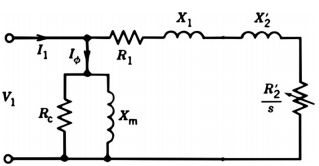
\includegraphics[scale=1.2]{imagens/15.PNG}
\caption{Circuito elétrico equivalente para a máquina de indução.}
\end{figure}


\subsubsection{Alimentação com tensão senoidal, frequência variável em regime permanente}
O motor de indução em regime permanente com alimentação senoidal pode ser representado pelo seguinte circuito conforme na figura \ref{fig:fig1-1}.

\begin{figure}[ht!]
\center
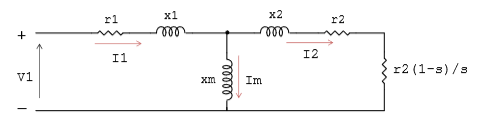
\includegraphics[scale= 0.88]{imagens/fig1-1.PNG}
\caption{\label{fig:fig1-1}Modelo em regime permanente senoidal para o motor de indução.}
\caption*{Fonte: MARTINS, eslaide 01 Acionamentos elétricos - Cap VIII}
\end{figure}

Note que\\

$r_{1}$ = resistência ôhmica do estator por fase;\\
$x_{1}$ = reatância de dispersão do estator por fase;\\
$r_{s}$ = resistência ôhmica do rotor por fase;\\
$x_{2}$ = reatância de dispersão do rotor por fase;\\
$w_{r}$ = frequência de pulsação das correntes do rotor;\\
$w_{s}$ = frequência de pulsação das correntes do estator;\\
$S$ = escorregamento do motor;\\
$V_{l} = V_{S}$ = tensão estatória por fase;\\

Para o cálculo do torque eletromagnético emprega-se o circuito da figura \ref{fig:fig1-1sss}.

\begin{figure}[ht!]
\center
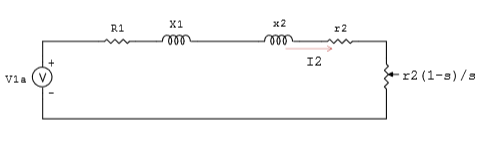
\includegraphics[scale= 0.88]{imagens/fig1-2.PNG}
\caption{\label{fig:fig1-1sss}Circuito equivalente para o cálculo do torque.}
\caption*{Fonte: MARTINS, eslaide 01 Acionamentos elétricos - Cap VIII}
\end{figure}

O torque eletromagnético é dado por:
\[T = \frac{1}{w_{sin}}\cdot \frac{q \cdot V_{1a}^2 \cdot \left ( \frac{r_{2}}{S} \right )}{\left [ \left ( R_{1} + \frac{r_{2}}{S}\right )^2 + \left ( X_{1}+x_{2} \right )^2\right ]}\]

Sabe-se que a velocidade de uma maquina síncrona é calculada sendo sessenta vezes a frequência do estator, dividido pelo numero de polos.
Além disso, sabe-se que a velocidade do rotor é aproximadamente igual a velocidade síncrona.
Assim, variando a frequência pode-se variar a velocidade da máquina. 
Por outro lado, o fluxo magnético é diretamente proporcional a tensão e inversamente a frequência. Logo, para variar a frequência deve-se variar a tensão.

O torque máximo desenvolvido pelo motor de indução, considerando impedância do estator desprezível é
\[T_{max} = k\cdot \phi_{S} ^2\]
O que mostra que o valor do torque máximo depende somente do fluxo no entreferro da maquina, não da frequência de operação.

Aproximando a frequência do estator com a frequência síncrona e fazendo algumas considerações obtém-se a equação do torque
\[T = \frac{p\cdot q}{r_{2}}\cdot \phi _S^2 \cdot w_{r}\]
O que demonstra que quando o fluxo é constante, com baixos valores de escorregamento, o torque é proporcional a pulsação rotórica.

A figura \ref{fig:fig1.3} ilustra as características torque/velocidade para um motor de indução com alimentação senoidal

\begin{figure}[ht!]
\center
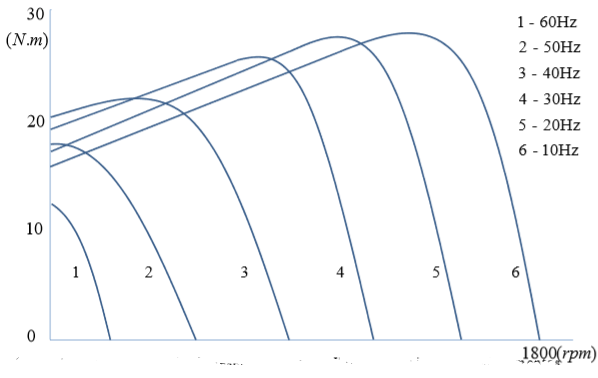
\includegraphics[scale= 0.88]{imagens/fig1-3.PNG}
\caption{\label{fig:fig1.3}Motor de indução com alimentação senoidal a frequência variável.}
\caption*{Fonte: MARTINS, eslaide 01 Acionamentos elétricos - Cap VIII}
\end{figure}

É visto que o torque máximo não é preservado quando V/f é constante. Assim em acionamentos melhores, emprega-se outra lei de fluxo, mais precisa.

A figura \ref{fig:fig1.4} mostra o fluxo magnetizante quando V/f é constante.

\begin{figure}[ht!]
\center
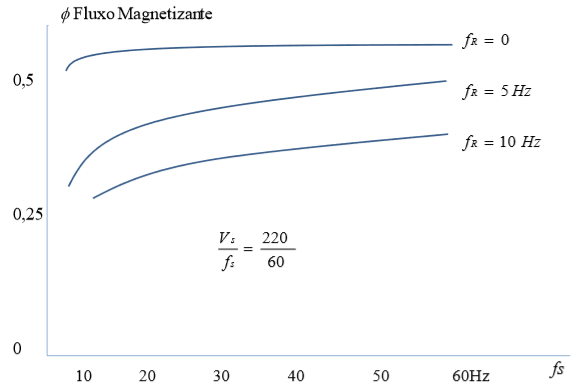
\includegraphics[scale= 0.88]{imagens/fig1-4.PNG}
\caption{\label{fig:fig1.4}Fluxo magnetizante em função da frequência de alimentação do estator e da frequência do rotor.}
\caption*{Fonte: MARTINS, eslaide 01 Acionamentos elétricos - Cap VIII}
\end{figure}

A figura \ref{fig:fig1.5} mostra o torque máximo quando V/f é constante.

\begin{figure}[ht!]
\center
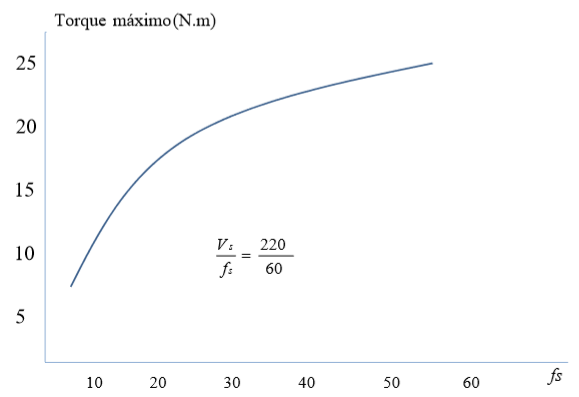
\includegraphics[scale= 0.88]{imagens/fig1-5.PNG}
\caption{\label{fig:fig1.5}Torque máximo em função da frequência de alimentação.}
\caption*{Fonte: MARTINS, eslaide 01 Acionamentos elétricos - Cap VIII}
\end{figure}

Observa-se que este método não pode ser empregado para cargas com altos torques em baixas velocidades.

Visto o modelo do motor de indução na forma complexa para alimentação senoidal em regime permanente, é estabelecida a lei V/f que permite manter o fluxo no entreferro constante.

\[\left | \bar{V_{s}} \right | = \frac{\left | \bar{\phi _{s}} \right | }{K_{s}}\cdot \sqrt{\frac{\left ( 1-w_{r}\cdot K_{r}\cdot w_{s}\cdot K_{s} \cdot \sigma\right )^2+\left ( w_{s}\cdot K_{s}+ w_{r}\cdot K_{r} \right )^2}{1+w_{r}^2\cdot K_{r}^2\cdot \sigma ^2}}\]

Assim, para que o fluxo se mantenha constante é necessário variar a tensão em função da frequência do estator e do rotor.
Simplificando a expressão através de considerações obtém-se:

\[\left( | \bar{V_{s}} \right) | = \left( | \bar{\phi _{s}} \right) \cdot w_{s}|\]

Que é a lei mais empregada devido a sua simplicidade.

\begin{figure}[ht!]
\center
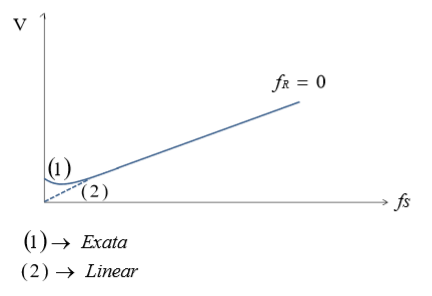
\includegraphics[scale= 0.88]{imagens/fig1-6.PNG}
\caption{\label{fig:fig1.6}Lei V/f para $f_{r}=0$}
\caption*{Fonte: MARTINS, eslaide 02 Acionamentos elétricos - Cap IX}
\end{figure}

A lei de fluxo exata em regime permanente, obtida através da equação da lei V/f para fluxo constante e de alguns parâmetros é representada no gráfico da figura \label{fig:fig1.7}.

\begin{figure}[ht!]
\center
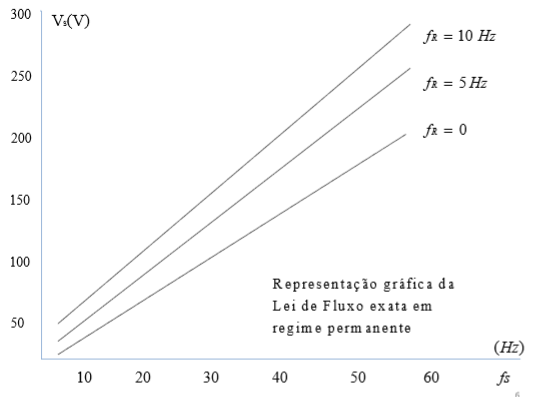
\includegraphics[scale= 0.88]{imagens/fig1-7.PNG}
\caption{\label{fig:fig1.7}Representação gráfica da lei de fluxo exata em regime permanente.}
\caption*{Fonte: MARTINS, eslaide 02 Acionamentos elétricos - Cap IX}
\end{figure}

A alimentação é direta, com fluxo constante, quando \[V_{s}/w_{s}\] é constante e \[w_{r}\] é variável.

\begin{figure}[ht!]
\center
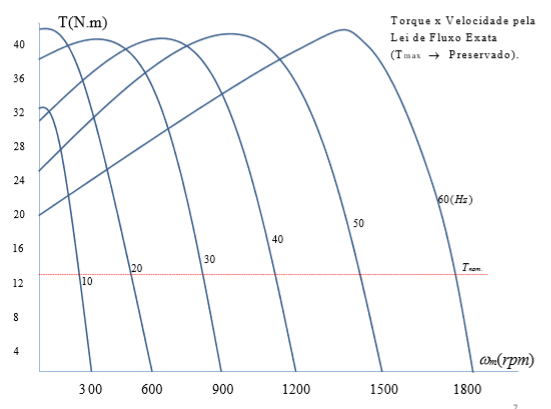
\includegraphics[scale= 0.88]{imagens/fig1-8.PNG}
\caption{\label{fig:fig1.8}Torque versos velocidade pela lei de fluxo correta.}
\caption*{Fonte: MARTINS, eslaide 02 Acionamentos elétricos - Cap IX}
\end{figure}

\begin{figure}[ht!]
\center
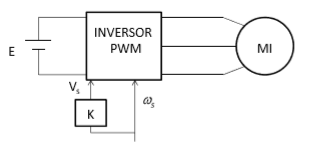
\includegraphics[scale= 0.88]{imagens/fig1-9.PNG}
\caption{\label{fig:fig1.9}Representação em blocos da alimentação direta.}
\caption*{Fonte: MARTINS, eslaide 02 Acionamentos elétricos - Cap IX}
\end{figure}

São vistas as características torque-velocidade.

\begin{figure}[ht!]
\center
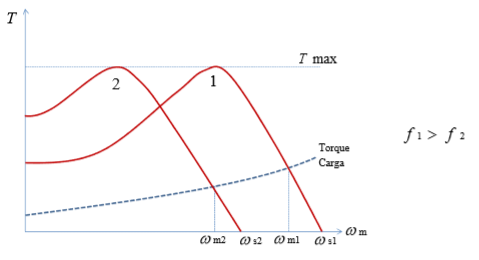
\includegraphics[scale= 0.88]{imagens/fig1-10.PNG}
\caption{\label{fig:fig1-10}Curva característica de torque-velocidade.}
\caption*{Fonte: MARTINS, eslaide 02 Acionamentos elétricos - Cap IX}
\end{figure}

A alimentação direta apresenta problemas fundamentais como a possibilidade de perda de estabilidade e possibilidade de haver solicitação excessiva de corrente do conversor.

\begin{figure}[ht!]
\center
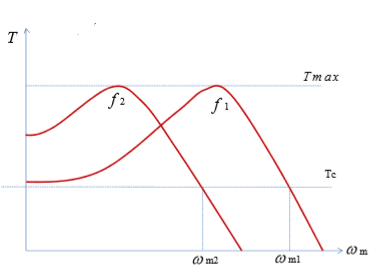
\includegraphics[scale= 0.88]{imagens/fig1-11.PNG}
\caption{\label{fig:fig1-11} Curva característica de torque-velocidade.}
\caption*{Fonte: MARTINS, eslaide 02 Acionamentos elétricos - Cap IX}
\end{figure}

A corrente pode assumir valores elevados no inversor e danificar o equipamento.

\begin{figure}[ht!]
\center
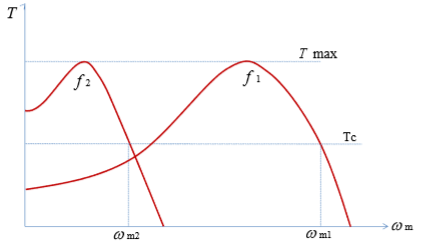
\includegraphics[scale= 0.88]{imagens/fig1-12.PNG}
\caption{\label{fig:fig1-12}Curva característica de torque-velocidade.}
\caption*{Fonte: MARTINS, eslaide 02 Acionamentos elétricos - Cap IX}
\end{figure}

Quando a frequência é subitamente alterada, o torque de carga torna-se maior que o elétrico e o motor bloqueia.

Para evitar esses problemas a máquina é alimentada com frequência de rotor imposto (auto-pilotagem).

\begin{figure}[ht!]
\center
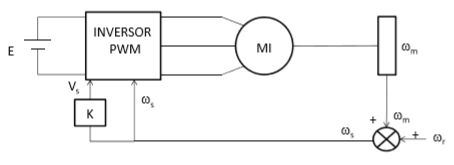
\includegraphics[scale= 0.88]{imagens/fig1-13.PNG}
\caption{\label{fig:fig1-13}Representação em blocos da auto-pilotagem.}
\caption*{Fonte: MARTINS, eslaide 02 Acionamentos elétricos - Cap IX}
\end{figure}

\begin{figure}[ht!]
\center
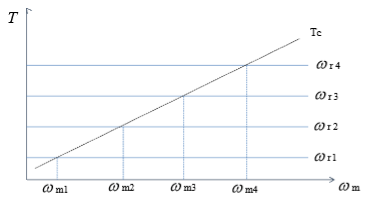
\includegraphics[scale= 0.88]{imagens/fig1-14.PNG}
\caption{\label{fig:fig1-14}Curva característica de torque-velocidade.}
\caption*{Fonte: MARTINS, eslaide 02 Acionamentos elétricos - Cap IX}
\end{figure}

A partir dos blocos da auto-pilotagem pode-se incluir um regulador de velocidade.

\begin{figure}[ht!]
\center
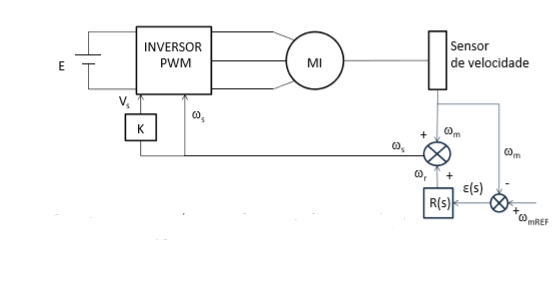
\includegraphics[scale= 0.88]{imagens/fig1-15.PNG}
\caption{\label{fig:fig1-15}Representação em blocos da auto-pilotagem com regulação de velocidade.}
\caption*{Fonte: MARTINS, eslaide 02 Acionamentos elétricos - Cap IX}
\end{figure}

Assim, agindo-se sobre o conversor causa-se uma variação na tensão E. Essa, por sua vez, é proporcional a frequência de funcionamento do inversor e com isso consegue-se manter a relação \[V_{s}/w_{s}\] constante.

\begin{figure}[ht!]
\center
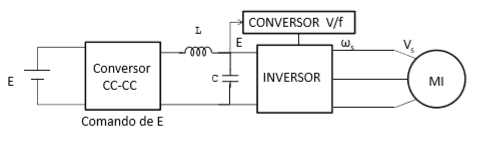
\includegraphics[scale= 0.88]{imagens/fig1-16.PNG}
\caption{\label{fig:fig1-16}Representação em blocos do controle indireto do torque máximo.}
\caption*{Fonte: MARTINS, eslaide 02 Acionamentos elétricos - Cap IX}
\end{figure}

Através de análise obtém-se
\[I_{cc} \approx K_{s}w_{r},\]
logo, limitando-se a corrente, limita-se a velocidade.

\begin{figure}[ht!]
\center
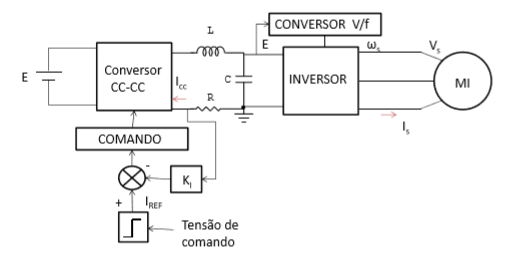
\includegraphics[scale= 0.88]{imagens/fig1-17.PNG}
\caption{\label{fig:fig1-17}Representação em blocos do controle indireto do torque máximo com limitação da corrente $I_{cc}$.}
\caption*{Fonte: MARTINS, eslaide 02 Acionamentos elétricos - Cap IX}
\end{figure}

Ainda, é possível controlar indiretamente a frequência retórica utilizando-se outro princípio. Partindo da equação do torque, através de considerações obtém-se que
\[\bar{I}_{1max} =  \bar{I}_{2max} + \bar{I}_{m}.\]
Portanto, limitando-se $\bar{I}_{2max}$, consequentemente de $w_{r}$ e do torque.

\begin{figure}[ht!]
\center
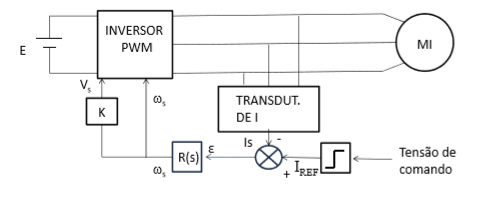
\includegraphics[scale= 0.88]{imagens/fig1-18.PNG}
\caption{\label{fig:fig1-18}Representação em blocos da auto-pilotagem com regulação de velocidade.}
\caption*{Fonte: MARTINS, eslaide 02 Acionamentos elétricos - Cap IX}
\end{figure}

\subsubsection{Corrente do estator e torque para alimentação retangular em tensão}

Quando o motor de indução, conectado em Y é alimentado por um inversor do tipo 180o, a tensão em cada uma das fases possui forma como visível na figura \ref{fig:fig21}.

\begin{figure}[ht!]
\center
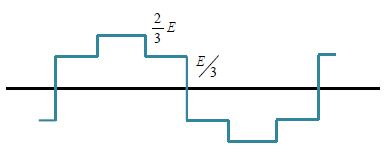
\includegraphics[scale= 0.88]{imagens/fig21.JPG}
\caption{\label{fig:fig21}Tensão aplicada a uma fase do estator.}
\caption*{Fonte: MARTINS, Acionamentos elétricos - Cap X.}
\end{figure}

A tensão de fase é
\[ v_{n}(t) = \frac{2E}{\pi }\cdot \frac{1}{n} \sin{nwt} \]

Os circuitos equivalentes são como na figura \ref{fig:fig22}.

\begin{figure}[ht!]
\center
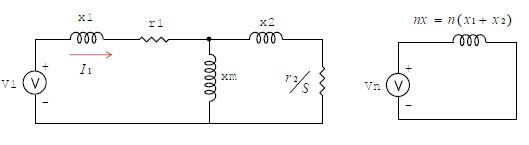
\includegraphics[scale= 0.88]{imagens/fig22.JPG}
\caption{\label{fig:fig22}Circuitos elétricos equivalentes para as tensão fundamental e harmônica.}
\caption*{Fonte: MARTINS, Acionamentos elétricos - Cap X.}
\end{figure}

A partir desses circuitos obtém-se

\[ i(t) = \frac{2E}{\pi }\left [ \frac{1}{\left | Z_{1} \right |} \sin{(wt-\theta _{1})} + \sum_{n=5}^{\infty } \frac{1}{n^2(x_{1}+x_2)} \sin{\left ( nwt-\frac{\pi }{2} \right )} \right ] \]

Empregando-se o método das harmônicas obtém-se

\begin{figure}[ht!]
\center
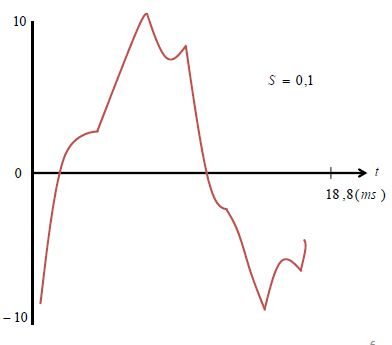
\includegraphics[scale= 0.88]{imagens/fig23.JPG}
\caption{\label{fig:fig23}Comportamento da corrente do motor com escorregamento de 0,1.}
\caption*{Fonte: MARTINS, Acionamentos elétricos - Cap X.}
\end{figure}

\begin{figure}[ht!]
\center
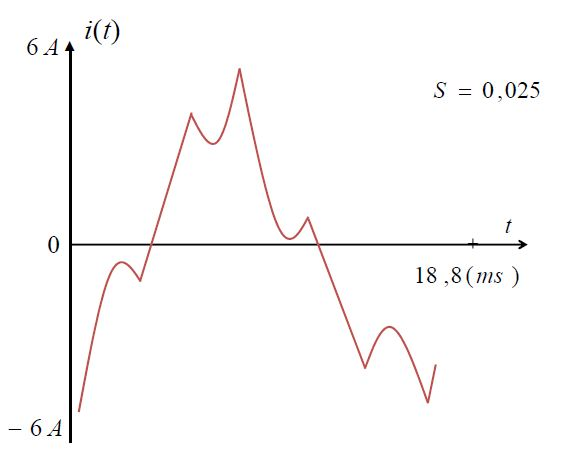
\includegraphics[scale= 0.88]{imagens/fig24.JPG}
\caption{\label{fig:fig24} Comportamento da corrente do motor com escorregamento de 0,025.}
\caption*{Fonte: MARTINS, Acionamentos elétricos - Cap X.}
\end{figure}

De acordo com o modelo para o motor de indução, na forma complexa, com o referencial fixo no estator do motor, após as devidas considerações, obtém-se
\[ T_e = T_{e_0} + \Delta T_e \]

Novamente, a tensão em cada uma das fases é

\begin{figure}[ht!]
\center
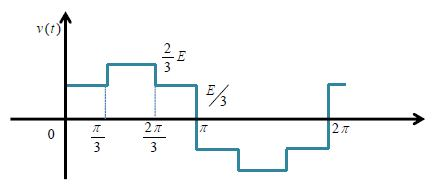
\includegraphics[scale= 0.88]{imagens/fig27.JPG}
\caption{\label{fig:fig27} Tensão de fase em um motor de indução trifásico ligado em Y.}
\caption*{Fonte: MARTINS, Acionamentos elétricos - Cap X.}
\end{figure}

O circuito equivalente das harmônicas é

\begin{figure}[ht!]
\center
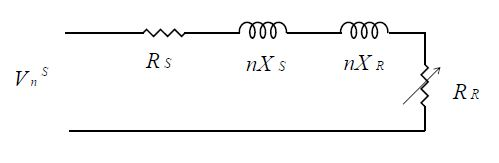
\includegraphics[scale= 0.88]{imagens/fig28.JPG}
\caption{\label{fig:fig28} Circuito equivalente para harmônicas de ordem n.}
\caption*{Fonte: MARTINS, Acionamentos elétricos - Cap X.}
\end{figure}

Cujos diagramas fasoriais são

\begin{figure}[ht!]
\center
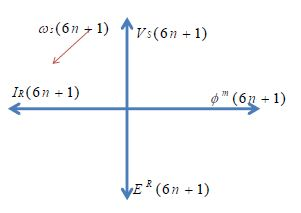
\includegraphics[scale= 0.88]{imagens/fig29.JPG}
\caption{\label{fig:fig29} Diagrama fasorial para as harmônicas (6n+1).}
\caption*{Fonte: MARTINS, Acionamentos elétricos - Cap X.}
\end{figure}

\begin{figure}[ht!]
\center
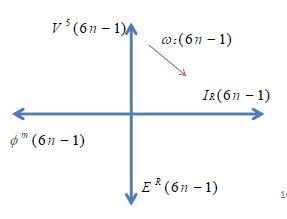
\includegraphics[scale= 0.88]{imagens/fig210.JPG}
\caption{\label{fig:fig210} Diagrama fasorial para as harmônicas (6n-1).}
\caption*{Fonte: MARTINS, Acionamentos elétricos - Cap X.}
\end{figure}

Então, calcula-se o torque pulsante

\[ T_6 = \frac{V_1 ^2}{w_s \cdot X_s}\frac{1}{50}  \]

Através de um exemplo, é possível ver que

\begin{figure}[ht!]
\center
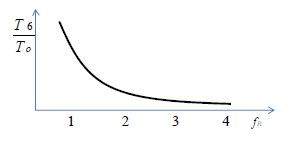
\includegraphics[scale= 0.88]{imagens/fig212.JPG}
\caption{\label{fig:fig212} Relação $T_{6}/T_{0}$ em função de $f_{r}$.}
\caption*{Fonte: MARTINS, Acionamentos elétricos - Cap X.}
\end{figure}

\begin{figure}[ht!]
\center
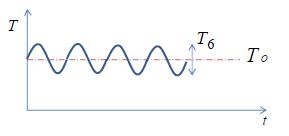
\includegraphics[scale= 0.88]{imagens/fig213.JPG}
\caption{\label{fig:fig213} Torque em função do tempo.}
\caption*{Fonte: MARTINS, Acionamentos elétricos - Cap X.}
\end{figure}

O torque pulsante tem amplitude constante, mas pode gerar oscilações no eixo do motor.

Consideramos o circuito equivalente do motor em regime permanente

\begin{figure}[ht!]
\center
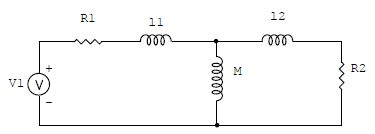
\includegraphics[scale= 0.88]{imagens/fig217.JPG}
\caption{\label{fig:fig217} Circuito elétrico equivalente em regime permanente.}
\caption*{Fonte: MARTINS, Acionamentos elétricos - Cap XI.}
\end{figure}

Para uma tensão de harmônica de ordem n o circuito equivalente adquire a configuração apresentada aqui

\begin{figure}[ht!]
\center
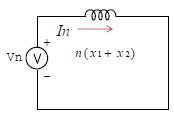
\includegraphics[scale= 0.88]{imagens/fig218.JPG}
\caption{\label{fig:fig218} Circuito equivalente do motor em regime permanente para as componentes harmônicas.}
\caption*{Fonte: MARTINS, Acionamentos elétricos - Cap XI.}
\end{figure}

Analisando o circuito, pode-se obter a equação da corrente eficaz

\[  I_{ef} = \sqrt{I_1 ^2 + \frac{V_1 ^2}{(x_1+x_2)^2}\sum_{n=5}^{\infty }\frac{1}{n^4}} \]

\begin{figure}[ht!]
\center
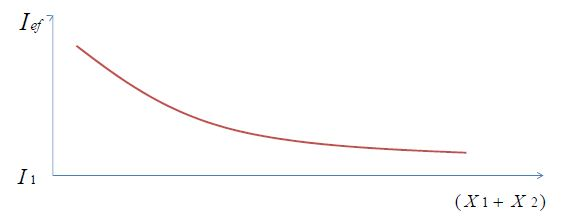
\includegraphics[scale= 0.88]{imagens/fig219.JPG}
\caption{\label{fig:fig219} $ I_{ef}$ em função de $(x_{1}+x_{2})$}
\caption*{Fonte: MARTINS, Acionamentos elétricos - Cap XI.}
\end{figure}

Para calculo da função de transferência considera-se o modelo

\begin{figure}[ht!]
\center
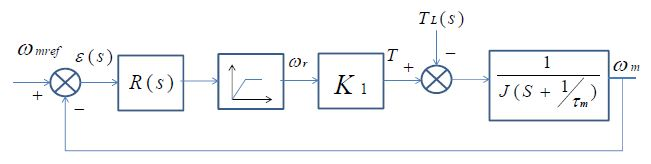
\includegraphics[scale= 0.88]{imagens/fig220.JPG}
\caption{\label{fig:fig220} Diagrama de blocos para estudo do comportamento dinâmico.}
\caption*{Fonte: MARTINS, Acionamentos elétricos - Cap XI.}
\end{figure}

Assim, obtém-se

\[ \frac{w_m(s)}{w_{m_{ref}}(s)} = \frac{K_1A}{J\left ( \frac{K_1A}{J}+\left ( s+ \frac{1}{\tau _m}\right ) \right )}  \]

que é a equação da função de transferência.

\subsubsection{Alimentação por corrente sob frequência variável em regime permanente - correntes senoidais}

Nesta seção será estudado o comportamento do motor de indução, em regime permanente, alimentado em corrente  e sob frequência variável. O modelo pode ser visto na figura \ref{fig:fig31}.

\begin{figure}[ht!]
\center
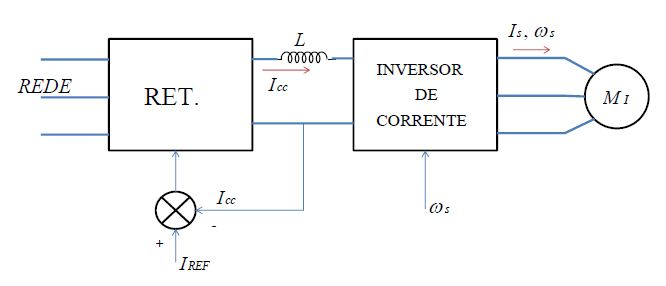
\includegraphics[scale= 0.88]{imagens/fig31.JPG}
\caption{\label{fig:fig31}Alimentação em corrente do motor de indução.}
\caption*{Fonte: MARTINS, Acionamentos elétricos - Cap XII.}
\end{figure}

O circuito equivalente para o modelo é da forma

\begin{figure}[ht!]
\center
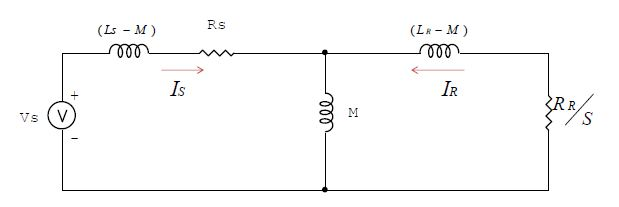
\includegraphics[scale= 0.88]{imagens/fig33.JPG}
\caption{\label{fig:fig33}Modelo em regime permanente senoidal para o motor de indução.}
\caption*{Fonte: MARTINS, Acionamentos elétricos - Cap XII.}
\end{figure}

Através da análise do circuito pela lei de malhas obtem-se que

\[ \phi _{s} = L_{s}\sqrt{\frac{R_{r}^2+(w_{r}L_{r}\sigma )^2}{R_{r}^2+(w_{r}L_{r} )^2}}\left | \bar{I}_{s} \right | \]

Assim, o fluxo do motor depende da frequência rotórica e da corrente estatórica, o que pode ser interpretado no circuito da figura \ref{fig:fig34}.

\begin{figure}[ht!]
\center
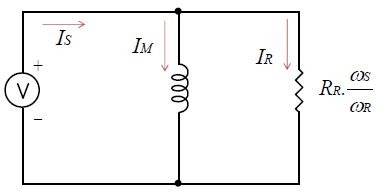
\includegraphics[scale= 0.88]{imagens/fig34.JPG}
\caption{\label{fig:fig34}Circuito equivalente simplificado.}
\caption*{Fonte: MARTINS, Acionamentos elétricos - Cap XII.}
\end{figure}

Após análise, obtém-se
\[ T=3p\frac{M^2w_r}{L_s\sqrt{R_r^2+w_r^2L_r^2}}\phi _sI_s  \]
que é representada na figura \ref{fig:fig35}.

\begin{figure}[ht!]
\center
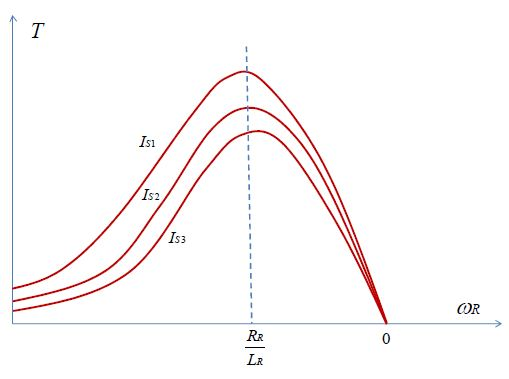
\includegraphics[scale= 0.88]{imagens/fig35.JPG}
\caption{\label{fig:fig35}Característica de torque/velocidade, tomando $ I_s $ como parâmetro.}
\caption*{Fonte: MARTINS, Acionamentos elétricos - Cap XII.}
\end{figure}

Considerando o sistema a seguir, impõe-se valores de $ I_s$ e de $ w_r $.

\begin{figure}[ht!]
\center
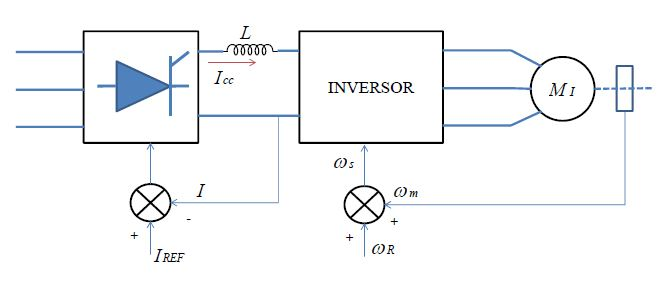
\includegraphics[scale= 0.88]{imagens/fig36.JPG}
\caption{\label{fig:fig36}Alimentação do motor com $ w_r$ imposto.}
\caption*{Fonte: MARTINS, Acionamentos elétricos - Cap XII.}
\end{figure}

Sabendo que
\[T = K_1 I_s^2\]
obtém-se
\[  \phi = K_2I_s \]
Logo, o torque e o fluxo independem da velocidade e dependem somente da corrente.

\begin{figure}[ht!]
\center
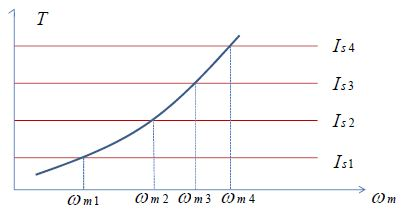
\includegraphics[scale= 0.88]{imagens/fig37.JPG}
\caption{\label{fig:fig37}Torque por velocidade para $  w_r $ constante.}
\caption*{Fonte: MARTINS, Acionamentos elétricos - Cap XII.}
\end{figure}

Entretanto, quando há saturação, o comportamento real do gráfico muda.

\begin{figure}[ht!]
\center
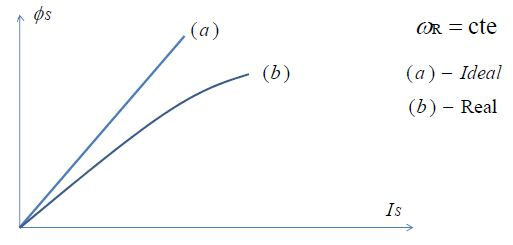
\includegraphics[scale= 0.88]{imagens/fig38.JPG}
\caption{\label{fig:fig38} Fluxo em função da corrente.}
\caption*{Fonte: MARTINS, Acionamentos elétricos - Cap XII.}
\end{figure}

\begin{figure}[ht!]
\center
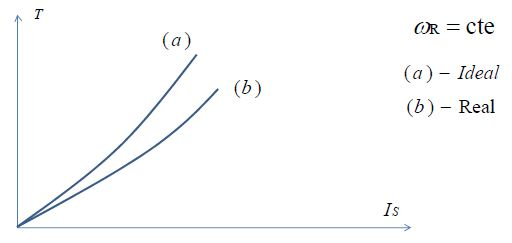
\includegraphics[scale= 0.88]{imagens/fig39.JPG}
\caption{\label{fig:fig39} Torque em função da corrente.}
\caption*{Fonte: MARTINS, Acionamentos elétricos - Cap XII.}
\end{figure}

A redução do torque reduz a potência no eixo, logo não é desejada.

Analisando agora em fluxo constante

\begin{figure}[ht!]
\center
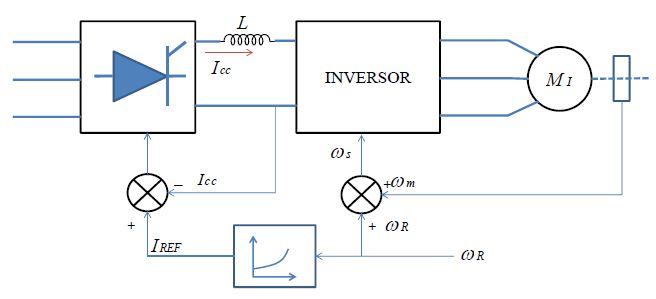
\includegraphics[scale= 0.88]{imagens/fig311.JPG}
\caption{\label{fig:fig311} Diagrama de blocos para manter o fluxo constante.}
\caption*{Fonte: MARTINS, Acionamentos elétricos - Cap XII.}
\end{figure}

Neste caso, o torque é dado por

\[  T = \frac{3p\phi _{s_{max}}^2}{R_r}w_r \]

O sistema usual para alimentação em corrente é representado na figura \ref{fig:fig312}.

\begin{figure}[ht!]
\center
\caption{\label{fig:fig312}Esquema de alimentação em corrente do motor de indução.}
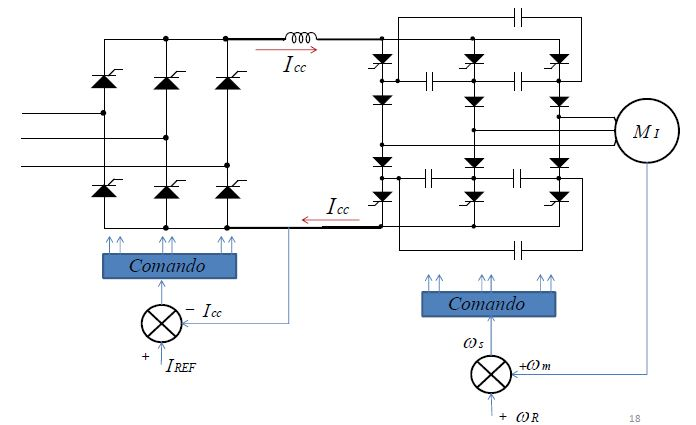
\includegraphics[scale= 0.80]{imagens/fig312.JPG}
\caption*{Fonte: MARTINS, Acionamentos elétricos - Cap XII.}
\end{figure}

\begin{figure}[ht!]
\center
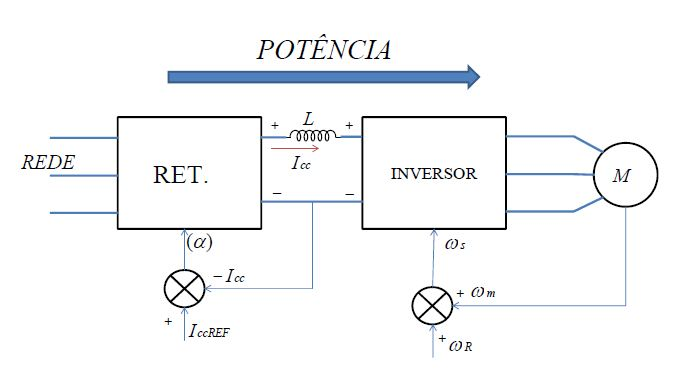
\includegraphics[scale= 0.88]{imagens/fig313.JPG}
\caption{\label{fig:fig313} Representação da tração.}
\caption*{Fonte: MARTINS, Acionamentos elétricos - Cap XII.}
\end{figure}

\begin{figure}[ht!]
\center
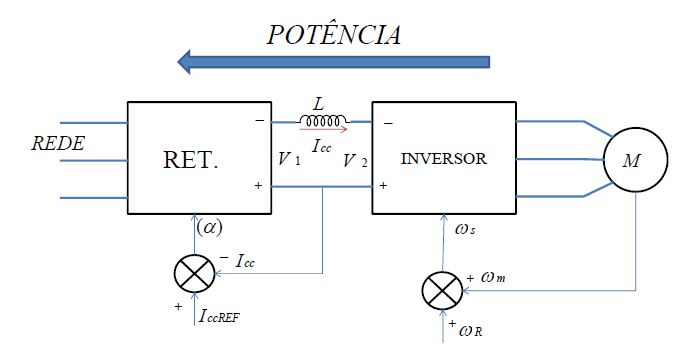
\includegraphics[scale= 0.8]{imagens/fig314.JPG}
\caption{\label{fig:fig314} Representação da frenagem.}
\caption*{Fonte: MARTINS, Acionamentos elétricos - Cap XII.}
\end{figure}

\begin{figure}[ht!]
\center
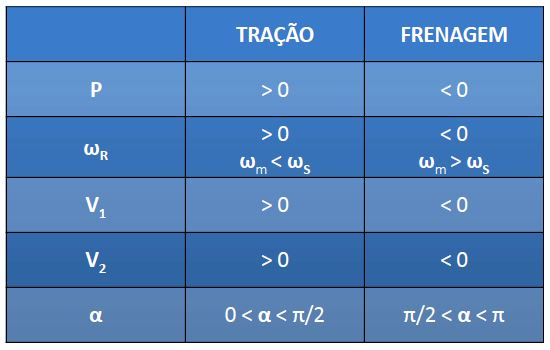
\includegraphics[scale= 0.88]{imagens/tab31.JPG}
\caption{\label{fig:tab31} Valores para a frenagem e tração.}
\caption*{Fonte: MARTINS, Acionamentos elétricos - Cap XII.}
\end{figure}

Para controlar a velocidade do motor é usado o diagrama representativo visto na figura \label{fig:fig315}.

\begin{figure}[ht!]
\center
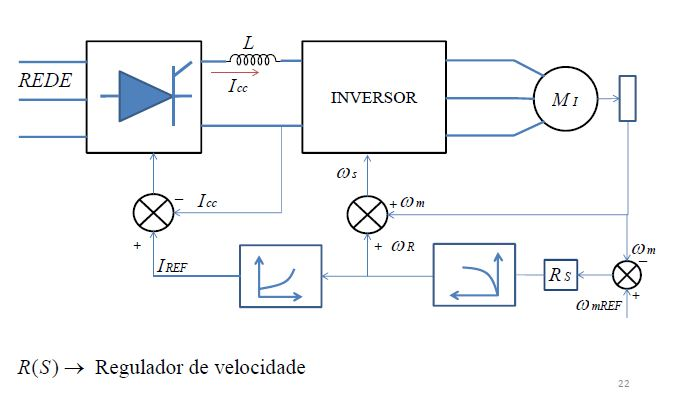
\includegraphics[scale= 0.88]{imagens/fig315.JPG}
\caption{\label{fig:fig315} Diagrama de blocos para o controle de velocidade.}
\caption*{Fonte: MARTINS, Acionamentos elétricos - Cap XII.}
\end{figure}

Para o exemplo de um motor particular,

\begin{figure}[ht!]
\center
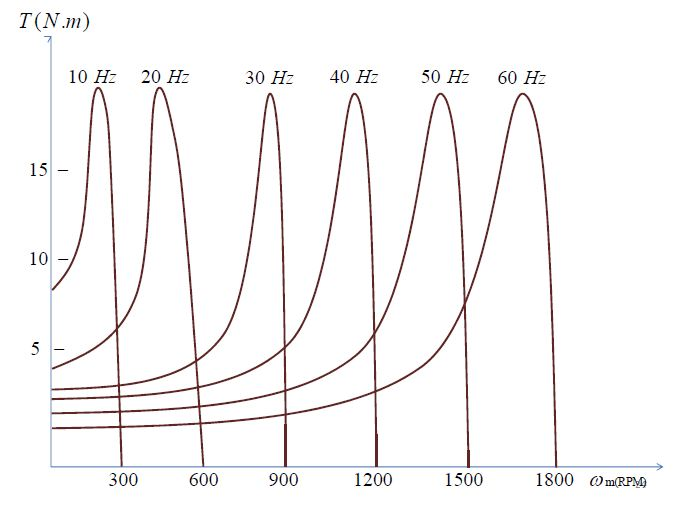
\includegraphics[scale= 0.88]{imagens/fig316.JPG}
\caption{\label{fig:fig316} Torque/velocidade do motor.}
\caption*{Fonte: MARTINS, Acionamentos elétricos - Cap XII.}
\end{figure}

\begin{figure}[ht!]
\center
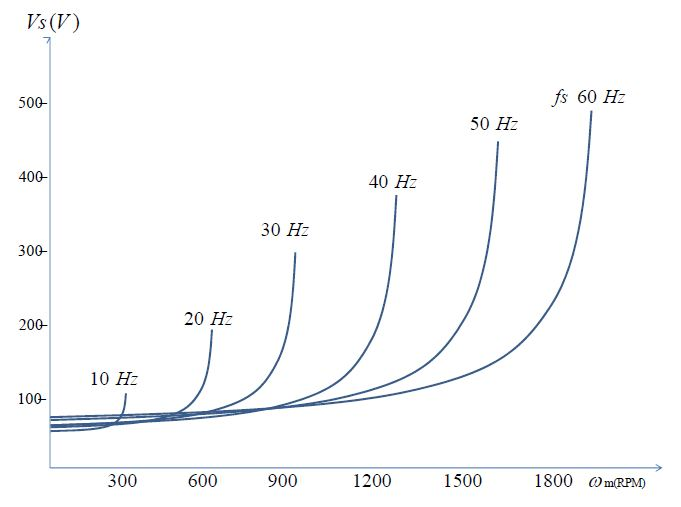
\includegraphics[scale= 0.75]{imagens/fig317.JPG}
\caption{\label{fig:fig317} Tensão de alimentação por velocidade do motor.}
\caption*{Fonte: MARTINS, Acionamentos elétricos - Cap XII.}
\end{figure}

\begin{figure}[ht!]
\center
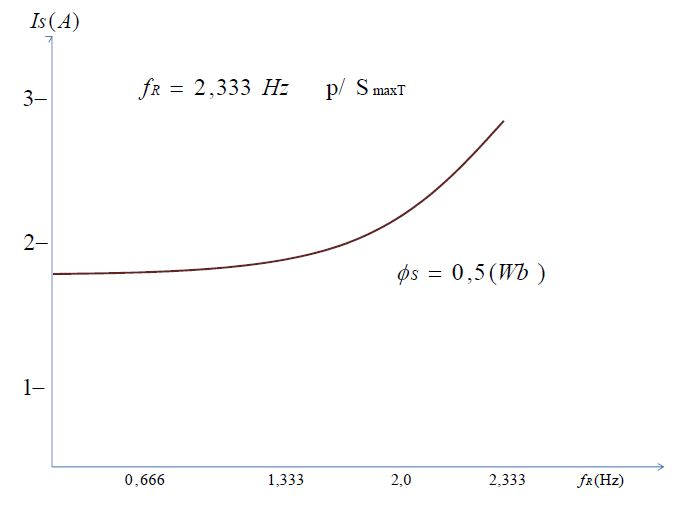
\includegraphics[scale= 0.88]{imagens/fig319.JPG}
\caption{\label{fig:fig319} Curva para baixos escorregamentos.}
\caption*{Fonte: MARTINS, Acionamentos elétricos - Cap XII.}
\end{figure}

\subsubsection{Alimentação por correntes retangulares}

Considerando a estrutura como na figura \ref{fig:fig41}.

\begin{figure}[ht!]
\center
\caption{\label{fig:fig41}Inversor de corrente alimentando um motor de indução conectado em $ \Delta $.}
\includegraphics[scale= 0.88]{imagens/fig41.JPG}
\caption*{Fonte: MARTINS, Acionamentos elétricos - Cap XIII.}
\end{figure}

A corrente em cada fase possui a forma

\begin{figure}[ht!]
\center
\includegraphics[scale= 0.88]{imagens/fig42.JPG}
\caption{\label{fig:fig42} Corrente idealizada em uma fase da máquina.}
\caption*{Fonte: MARTINS, Acionamentos elétricos - Cap XIII.}
\end{figure}

Analisando expressão obtém-se o valor do torque médio
\[ T = 3p\frac{w_rR_rM^2}{R_r^2+w_r^2L_r^2}I_{1ef}^2  \]
e também
\[ \frac{\Delta T_{max}}{T} = \frac{1}{3w_r \tau _r}  \], onde \[  \tau _r = \frac{L_r}{R_r} \]

As figuras a seguir mostram as sequências de comutação da corrente que alimenta o motor.

\begin{figure}[ht!]
\center
\includegraphics[scale= 0.88]{imagens/fig45.JPG}
\caption{\label{fig:fig45} Antes da comutação.}
\caption*{Fonte: MARTINS, Acionamentos elétricos - Cap XIII.}
\end{figure}


\begin{figure}[ht!]
\center
\includegraphics[scale= 0.88]{imagens/fig46.JPG}
\caption{\label{fig:fig46} Primeira etapa da comutação.}
\caption*{Fonte: MARTINS, Acionamentos elétricos - Cap XIII.}
\end{figure}


\begin{figure}[ht!]
\center
\includegraphics[scale= 0.88]{imagens/fig47.JPG}
\caption{\label{fig:fig47} Segunda etapa da comutação.}
\caption*{Fonte: MARTINS, Acionamentos elétricos - Cap XIII.}
\end{figure}


\begin{figure}[ht!]
\center
\includegraphics[scale= 0.88]{imagens/fig48.JPG}
\caption{\label{fig:fig48} Após a comutação.}
\caption*{Fonte: MARTINS, Acionamentos elétricos - Cap XIII.}
\end{figure}

Durante o segundo intervalo de comutação, o capacitor está associado ao motor, como visto a seguir.

\begin{figure}[ht!]
\center
\includegraphics[scale= 0.88]{imagens/fig413.JPG}
\caption{\label{fig:fig413} Circuito elétrico equivalente.}
\caption*{Fonte: MARTINS, Acionamentos elétricos - Cap XIII.}
\end{figure}

Então a pulsação natural do circuito durante o intervalo é dado por
\[ w_0 \sqrt{\frac{3}{2lC}}  \]

Considerando o gráfico

\begin{figure}[ht!]
\center
\includegraphics[scale= 0.88]{imagens/fig414.JPG}
\caption{\label{fig:fig414} Tensão e corrente no capacitor de auxílio de comutação.}
\caption*{Fonte: MARTINS, Acionamentos elétricos - Cap XIII.}
\end{figure}

Obtém-se
\[ \tau _2 = \frac{\pi }{2}\sqrt{\frac{2lC}{3}}  \]

As correntes de fase estão representadas a seguir

\begin{figure}[ht!]
\center
\includegraphics[scale= 0.88]{imagens/fig415.JPG}
\caption{\label{fig:fig415} Correntes de fase no motor durante a comutação.}
\caption*{Fonte: MARTINS, Acionamentos elétricos - Cap XIII.}
\end{figure}

Em consequência da rápida variação da corrente, a tensão apresenta picos nesses intervalos, como vistos na figura

\begin{figure}[ht!]
\center
\includegraphics[scale= 0.88]{imagens/fig419.JPG}
\caption{\label{fig:fig419} Picos de tensão devido a variação da corrente.}
\caption*{Fonte: MARTINS, Acionamentos elétricos - Cap XIII.}
\end{figure}

Após análise, conclui-se que os picos crescem linearmente com a corrente e que quanto maior a indutância de dispersão maior os valores das tensões de pico.
Logo, na alimentação em corrente usa-se motores com baixa indutância de dispersão, o contrário do que se deseja em motores alimentados em tensão.

\subsubsection{Controle de velocidade com um gradador}

Conhecida a equação do torque sabe-se que para um escorregamento dado, o torque produzido é proporcional ao quadrado da tensão estatória.

\begin{figure}[ht!]
\center
\includegraphics[scale= 0.88]{imagens/fig51.JPG}
\caption{\label{fig:fig51} Curva de torque por escorregamento.}
\caption*{Fonte: MARTINS, Acionamentos elétricos - Cap XIV.}
\end{figure}

Assim, a variação da tensão estatória é um método de controle de velocidade do motor. Classicamente, usa-se autotransformadores.

\begin{figure}[ht!]
\center
\includegraphics[scale= 0.88]{imagens/fig52.JPG}
\caption{\label{fig:fig52} Motor alimentado por autotransformador.}
\caption*{Fonte: MARTINS, Acionamentos elétricos - Cap XIV.}
\end{figure}

Entretanto, esses são ruins e difíceis de automatizar. Logo, a solução é o uso de gradadores.

\begin{figure}[ht!]
\center
\includegraphics[scale= 0.88]{imagens/fig53.JPG}
\caption{\label{fig:fig53} Gradador monofásico alimentando uma carga resistiva.}
\caption*{Fonte: MARTINS, Acionamentos elétricos - Cap XIV.}
\end{figure}

Como visto no exemplo a seguir.

\begin{figure}[ht!]
\center
\includegraphics[scale= 0.88]{imagens/fig54.JPG}
\caption{\label{fig:fig54} Gradador trifásico alimentado um motor de indução trifásico.}
\caption*{Fonte: MARTINS, Acionamentos elétricos - Cap XIV.}
\end{figure}

O gradador, em geral, é usado somente para realizar a partida do motor. Esse processo é chamado de soft-start.

